\documentclass[border=2pt]{standalone}

% Drawing
\usepackage{tikz}

% Tikz Library
\usetikzlibrary{decorations.markings, calc, shapes.geometric, angles, quotes, shapes, calc}

% Styles
%% Incident Ray
\tikzstyle{ray} = [%
					line width = 0.85, 
					color = red,
					postaction = decorate, decoration={markings, mark=at position .52 with \arrow{stealth}}
					]
%% Refracted Ray
\tikzstyle{ray1} = [%
					line width = 0.85, 
					color = red]
%% Dashed
\tikzstyle{vertical} = [%
					line width = 0.85, 
					dashed]

\usetikzlibrary{backgrounds}

\begin{document}
		
	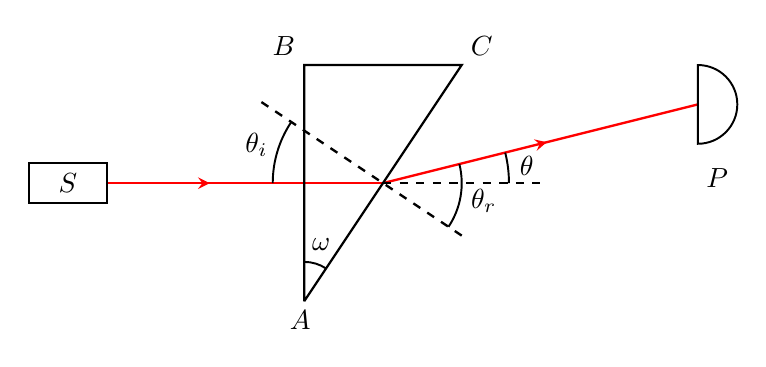
\begin{tikzpicture}[semic/.style args={#1,#2}{semicircle,minimum width=#1,draw,anchor=arc end,rotate=#2},outer sep=0pt,line width=.7pt]
		
		% Grid
%		\draw[dotted] (0,0) grid (10,10);
%		\foreach \i in {0,...,10}
%		{
%			\node at (-2ex,\i) {\i};
%			\node at (\i,-2ex) {\i};
%		}
		
		% Coordinates
		\coordinate (S) at (1,1.5);
		\coordinate (P) at (9,3);
		\coordinate (A) at (4,1.5);
		\coordinate (B) at (5,1.5);
		\coordinate (C) at (6, 29/6-4);
		\coordinate (C') at (3.4, 2.56667);
		
		% Nodes
		%% Source
		\node[draw, rectangle, minimum width=1cm, minimum height=0.5cm] at (S) (s) {$S$};
		%% Detector
		\node [semic={1cm,-90}, label={[rotate=0, below left, yshift=-0.7cm]$P$}] at (P) {};
		
		% Prism
		\draw[thick] (4,0) coordinate (K) node [below, xshift=-0.05cm] {$A$} -- ++(0,3) coordinate (L) node [above left] {$B$}-- +(2,0) coordinate (M) node [above right] {$C$} -- (4,0);
		
		
		\begin{scope}[on background layer]
			% Rays
			\draw[ray] (s) -- (A);
			\draw[ray] (B) -- (9,2.5) coordinate (P');
			\draw[ray1] (A) -- (B);
			% Dashed
			\draw[vertical] (C) -- (C');
			\draw[vertical] (B) -- (7,1.5) coordinate (B');
		\end{scope}
		
		% Angles
		\pic[draw, "$\omega$", angle eccentricity=1.5] {angle={M--K--L}};
		\pic[draw, "$\theta_i$", angle eccentricity=1.2, angle radius=1.4cm] {angle={C'--B--S}};
		\pic[draw, "$\theta_r$", angle eccentricity=1.3, angle radius=1cm] {angle={C--B--P'}};
		\pic[draw, "$\theta$", angle eccentricity=1.15, angle radius=1.6cm] {angle={B'--B--P'}};
	\end{tikzpicture}
	
\end{document}
